% ------------------------------------------------------------------------------
% TYPO3 CMS 8 LTS - What's New - Chapter "Install Tool" (Dutch Version)
%
% @author	Michael Schams <schams.net>
% @license	Creative Commons BY-NC-SA 3.0
% @link		http://typo3.org/download/release-notes/whats-new/
% @language	English
% ------------------------------------------------------------------------------
% LTXE-CHAPTER-UID:		c2b5a740-582cc152-17e7619f-b938f624
% LTXE-CHAPTER-NAME:	Install Tool
% ------------------------------------------------------------------------------

\section{Install Tool}
\begin{frame}[fragile]
	\frametitle{Install Tool}

	\begin{center}\huge{\color{typo3darkgrey}\textbf{Install Tool}}\end{center}
	\begin{center}\large{\textit{Krachtig gereedschap voor integrators en ontwikkelaars}}\end{center}

\end{frame}

% ------------------------------------------------------------------------------
% LTXE-SLIDE-START
% LTXE-SLIDE-UID:		f5eeca9a-8d339294-399ba4bc-96adacb0
% LTXE-SLIDE-ORIGIN:	f6668b2d-8932a470-5b9c024c-e4e9f53a English
% LTXE-SLIDE-TITLE:		Install Tool: Upgrade Analysis
% ------------------------------------------------------------------------------

\begin{frame}[fragile]
	\frametitle{Install Tool}
	\framesubtitle{Upgrade Analyse}

% The install tool, which is also a heavily used feature during updates between
% TYPO3 versions, has received some more beauty, basically finding all documented
% changes with a cool filter to show what is relevant for an integrator,
% extension author or site owner. Although this is already pretty cool, stay
% tuned for even better features to make migrations even easier between TYPO3
% versions!
% The migration and deprecation of existing options and switching within the TCA
% definitions we have in place since TYPO3 v7, is also visible in the Install Tool
% now.

	TYPO3 upgrades eenvoudig door de nieuwe \textbf{Upgrade Analyse} tool
	in de Install Tool (zoeken/filteren van gedocumenteerde wijzigingen tussen versies).

	\begin{figure}
		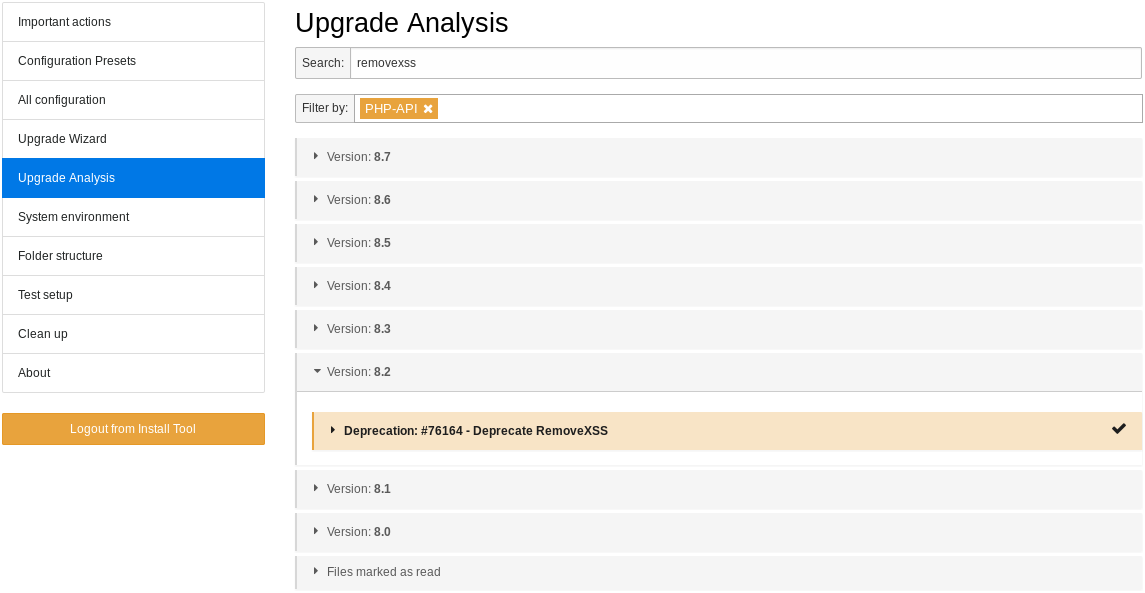
\includegraphics[width=0.7\linewidth]{InstallTool/install-tool-upgrade-analysis.png}
	\end{figure}

\end{frame}

% ------------------------------------------------------------------------------
% LTXE-SLIDE-START
% LTXE-SLIDE-UID:		0112aad3-5c793015-ea26a88e-201db3a1
% LTXE-SLIDE-ORIGIN:	9702aaf4-f02bbc35-67902b2e-42855506 English
% LTXE-SLIDE-TITLE:		Install Tool: Upgrade Analysis
% LTXE-SLIDE-REFERENCE:	#78222: Dump Class Loading Information UI in Install Tool
% ------------------------------------------------------------------------------

\begin{frame}[fragile]
	\frametitle{Install Tool}
	\framesubtitle{Autoload-informatie dumpen}

	Om de informatie voor het laden van klassen te herbouwen is een nieuwe actie
	toegevoegd aan de Install Tool om autoload-informatie te dumpen.

	\begin{figure}
		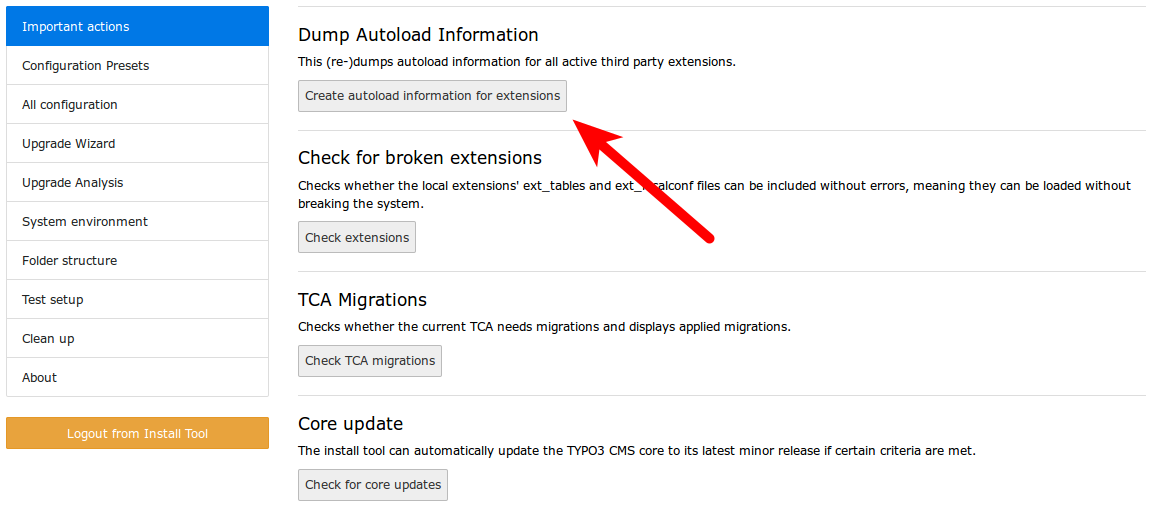
\includegraphics[width=0.8\linewidth]{InstallTool/78222.png}
	\end{figure}

\end{frame}

% ------------------------------------------------------------------------------
% LTXE-SLIDE-START
% LTXE-SLIDE-UID:		fe2580ff-71dd148b-e0e59897-64161ff0
% LTXE-SLIDE-ORIGIN:	5a194e82-8eac7f1b-ef2730da-61d781b2 English
% LTXE-SLIDE-TITLE:		Install Tool: TCA Migration Messages
% ------------------------------------------------------------------------------

\begin{frame}[fragile]
	\frametitle{Install Tool}
	\framesubtitle{TCA migratieberichten}

	TCA migratieberichten kunnen nu bekeken worden in de Install Tool.

	\begin{figure}
		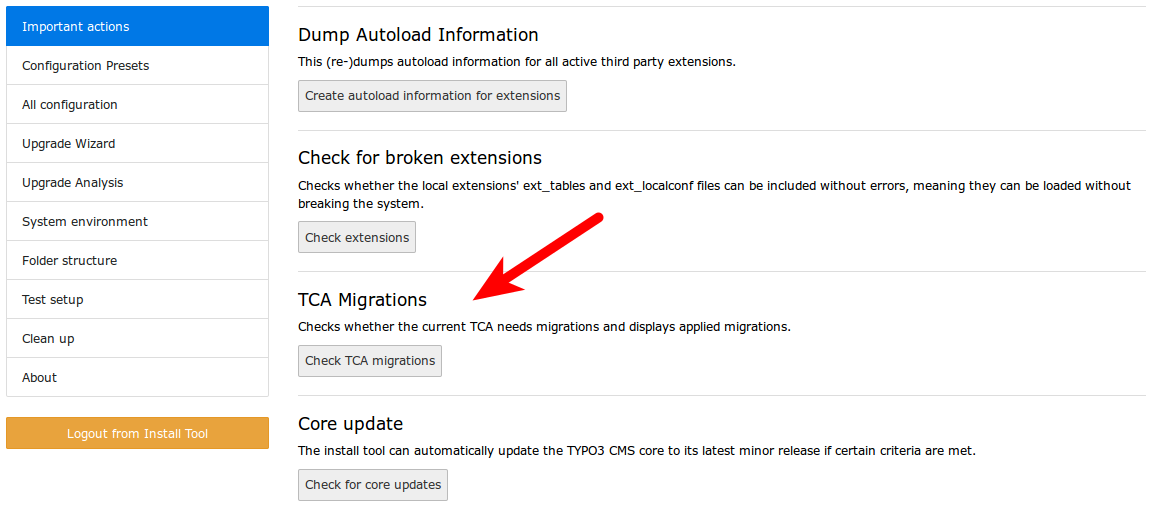
\includegraphics[width=0.8\linewidth]{InstallTool/77799.png}
	\end{figure}

\end{frame}


% ------------------------------------------------------------------------------
% LTXE-SLIDE-START
% LTXE-SLIDE-UID:		56483bd4-d1147d07-4e0b268e-4cca435e
% LTXE-SLIDE-ORIGIN:	8b1a9661-d6fab90f-9c856224-ee663aa2 English
% LTXE-SLIDE-TITLE:		#77757: Re-check if an UpdateWizard should run
% ------------------------------------------------------------------------------
\begin{frame}[fragile]
	\frametitle{Systeemwijzigingen}
	\framesubtitle{Update-assistent}

	\begin{columns}[T]
		\begin{column}{.5\textwidth}
			De Update-assistent in de Install Tool geeft een overzicht van taken die \textit{afgerond} zijn.
			\newline\newline
			Keuzevakjes en een knop "Recheck chosen wizards" zorgen ervoor dat updates opnieuw uitgevoerd kunnen worden.
			De assistent test zelf of de taak opnieuw uitgevoerd moet worden.
		\end{column}
		\begin{column}{.5\textwidth}
			\begin{figure}\vspace*{-0.5cm}
				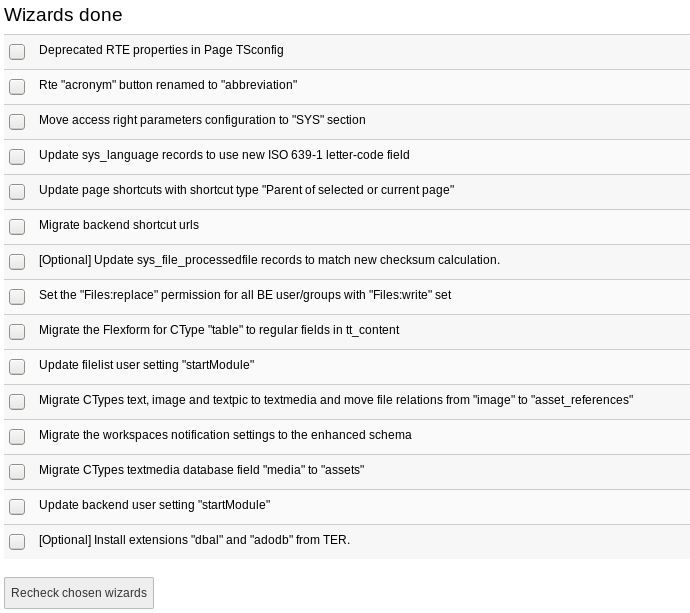
\includegraphics[width=0.8\linewidth]{InstallTool/77757.png}
			\end{figure}
		\end{column}
	\end{columns}

\end{frame}


% ------------------------------------------------------------------------------
